
% this file is called up by thesis.tex
% content in this file will be fed into the main document

%: ----------------------- introduction file header -----------------------
\begin{savequote}[50mm]
% I think most people just make the mistake that it should be simple to design simple things
The effort required to design something is inversely proportional to the simplicity of the result.% As architectural styles go, REST is very simple.
\qauthor{Roy T. Fielding} % puede ser una cita muy gallita, como presumiendo que lo mio es simple
                          % o justo todo lo contrario: lo mio no es sencillo, luego no te habrá supuesto mucho esfuerzo
\end{savequote}


\newcommand{\codigo}[1]{``\texttt{#1}''}
\newcommand{\primquery}{\emph{query}}
\newcommand{\primread}{\emph{read}}
\newcommand{\primtake}{\emph{take}}
\newcommand{\primwrite}{\emph{write}}


\chapter{Triple Space Computing for resource constrained devices}
\label{cha:tsc}
\newcommand{\pathchapthree}{3_tsc}

% the code below specifies where the figures are stored
\ifpdf
    \graphicspath{{\pathchapthree/figures/PNG/}{\pathchapthree/figures/PDF/}{\pathchapthree/figures/}}
\else
    \graphicspath{{\pathchapthree/figures/EPS/}{\pathchapthree/figures/}}
\fi



% ----------------------------------------------------------------------


In recent years, the \acf{iot} has became a reality due to the increasing number of everyday objects equipped with computing and networking capabilities.
The use of these objects together with the rising of mobile computing greatly contributes to the \ac{ubicomp} vision.
%In the beginning the community put more effort on those devices' connectivity issues, materialized in the spread of technologies such as Zigbee\footnote{http://www.zigbee.org}, 6LoWPAN\footnote{http://datatracker.ietf.org/wg/6lowpan/charter/} or Bluetooth\footnote{http://www.bluetooth.com}.
%However, nowadays it is focusing on the architectural solutions used by the applications built around these objects.
%A classification of these solutions has been already presented in the previous chapter. % Coulouris et al.
In this thesis, we defend that \acf{tsc} provides some valuable properties to \ac{ubicomp} environments. % mencionarlas?
However, some other properties are derived from how \ac{tsc} is implemented. % TODO implemented suena muy umpa-lumpa? mejor designed o así? o hablar de model mejor que de middleware?


% TODO problema: y por qué no otros? Habría que redactarlo de tal forma que no haga que un lector tiquismiquis requiera un puto survey de network-based architectural styles!
In this chapter we focus on selecting the underlying network-based architectural style.
Particularly, we analyze the widely adopted \acf{rest}.
Its application to resource constrained devices brought the successful \ac{wot} initiative.
\ac{wot} is probably the most prominent architectural solution used for smart-objects. % probably porque no tengo datos que lo defiendan
%The benefits that \ac{rest} brings to resource constrained devices have been deeply described in the previous chapter.


To that end, Section~\ref{sec:tsc_restfulness} analyzes the characteristics of the \ac{rest} architectural style and the similarities it shares with \ac{tsc}.
Later, it describes a \ac{rest}-like \ac{api} to access a triplespace. % TODO ver cómo escribir triplespace
The goal pursued is two-fold: (1) inherit valuable the properties from \ac{rest} and (2) maintain a high degree of compatibility with the \ac{wot}.
Section~\ref{sec:distributed_tsc} presents the need and requirements of a distributed architecture for \ac{ubicomp}.
These requirements lead us to adapt the \ac{tsc} model.
Finally, Section~\ref{sec:middleware_qualitative_evaluation} evaluates the properties achieved with this model.


%    propiedades aportadas por REST a IoT

\section{On the \acs{rest}fulness of \acs{tsc}}
\label{sec:tsc_restfulness}

\subsection{\acl{rest}}
\label{sec:rest}

\acf{rest} is a network-based architectural style proposed by \citet{fielding_architectural_2000}.
% descripción de propiedades de REST: hipermedia distribuído
% que es hipertexto? http://roy.gbiv.com/untangled/2008/rest-apis-must-be-hypertext-driven#comment-718
It aims to cover certain properties, explained in Section~\ref{sec:network_properties}.
% Estilos de los que se deriva: ¿?
To achieve these properties, \ac{rest} establishes the following constraints from other network-based architectural styles:
% explicarlo o es demasiado obvio?
\begin{description}
 \item[\acf{rest_cs}.] Providing an \ac{api} to the clients, they are isolated from back-end implementation details.
		       % esto ayuda a: , scalability, evolvability (apps independientes pueden evolucionar mejor)
 \item[\acf{rest_s}.] The state is fully stored in the client and therefore each request has all the information needed to process it.
 \item[\acf{rest_cache}.] When added to the \ac{rest_cs} constraint, this style replicates content obtained from a server in the client.
 \item[\acf{rest_u}.] It is the key constraint which distinguishes \ac{rest} from other architectural styles.
                      This constraint is composed by the following ones:
    \begin{description}
	% explicados en sección 5.2 de Fielding, resumir?
	\item[\acf{rest_id}.] Resources are the conceptual targets of hypertext references.
			      Their identification offers a generic interface to access and change the values of a resource.
	\item[\acf{rest_rep}.] Representations are composed by a sequence of bytes and the metadata to describe those bytes.
	\item[\acf{rest_desc}.] The client and server have to agree on standard methods and media types. % linkar al tipo de la Web esa
				% Explicación Fielding:
				% interaction is stateless between requests
				% standard methods and media types are used to indicate semantics and exchange information
				% responses explicitly indicate cacheability.
		                %\ac{http}'s content negotiation for instance, allows to reach an agreement on the media types.
	                        Beyond that point, each request or response should contain all the needed data to process it.
	                        Therefore, in \citeauthor{fielding_architectural_2000}'s words,
	                        the type should be registered,
	                        the registry should point to a specification and 
	                        the specification should explain how to process data according to its intent \citep{wahbe_self-descriptive_2010}. % no necesariamente tiene que ser estándar
	\item[\acf{rest_hateoas}.] This is a controversial constraint because most of the self-proclaimed ``\ac{rest}'' \acp{api} fail to follow it \citep{house_how_2012}.
	                           It states that no out-of-the-band information should guide the interaction with an \ac{api}.
	                           Instead, the hypertext should guide it.
	                           In other words, the client must know just an initial URL and the application's media types.
	                           From that point, it should select the alternatives proposed by the server to change to the next application state \citep{fielding_rest_2008}.
	                           % propuestas: respresentaciones (links) y la manipulación implicita de las mismas (CRUD)
    \end{description}
 \item[\acf{rest_l}.] Each layer provides services to the top layer. % e.g. TCP/IP
 \item[\acf{rest_cod}.] The client has a set of resources which does not know how to process.
                        This \emph{know-how} is downloaded from the server.
\end{description}


\subsection{Suitable Protocols for \ac{rest}}
\label{sec:protocols}

% sólo por el correcto uso de ciertos protocolos se puede conseguir todo menos HATEOAS => citar el vídeo aquel

% hablar un poco de HTTP y CoAP y decir por qué no hablamos más a menudo de CoAP

Historically, \acf{http} has been considered a suitable protocol to follow the \ac{rest} style. % TODO cite
\ac{http} is a simple protocol whose adoption by computing platforms is massive.


However, in the last few years \acf{coap} has emerged as a specialized web transfer protocol for resource constrained devices. % has emerged, has arisen?
Some noteworthy features of \ac{coap} are
(1) the reduced message size,
(2) the use of UDP as a transport layer (with the possibility of using \emph{multicast} communication),
(3) similarity with \ac{http} (both to reuse its properties and to ease cross-protocol proxying),
(4) a resource discovery mechanism. % TODO cita a CORE
% mencionar seguridad?


One could defend that to design a lightweight \ac{tsc} solution \ac{coap} should be used as a baseline.
However, we have chosen to work with \ac{http} for the following reasons:
\begin{itemize}
  \item RDF-based media-formats can be rather verbosed.
	This contrasts with \ac{coap}'s message size limitations.
	Dealing with this limitations was not one main goals of the thesis.
	However, we have considered them at some points of the dissertation to avoid unrealistic assumptions.
  \item \ac{coap} is an ongoing standard.
        Therefore, its definition slightly changes in each draft version.
        A practical limitation of this is that at the moment there are few libraries
        and tools to work with \ac{coap}.
        This limits the range of platforms which could adopt any solution proposed.
  \item Due to its similarities with \ac{coap}, the future adoption of the latter should be relatively straightforward.
        % sin contar con los aspectos destacados anteriormente
\end{itemize}

% Ideas no usadas:
% REST no dice nada, pero de facto el protocolo es HTTP
% durante el desarrollo de esta tesis en resource constrained ha surgido CoAP
%   muchas de las cosas aquí comentadas son iguales o mejor sobre CoAP
%   de todas formas, ha habido algo que ha guiado nuestro diseño: librerias existentes => afecta a plataformas
%         si, pero para eso está lo de layered approach! => motivos prácticos



\subsection{\acl{tsc}}
\label{sec:tsc_vs_rest}

\ac{tsc} consist of a shared space which is accessed using some known primitives.
\emph{Per se}, \ac{tsc} does not contradict in any sense the \ac{rest} principles:

\begin{description}
 \item[\ac{rest_cs}.] Providing the access to each space is centralized in a machine, clients can access to it using \emph{CS}.
           This does not prevent to use a distributed semantic repository in the backend.
 \item[\ac{rest_s}.] The primitives to access the space imply simple read and writes which do not store any state in the server.
 \item[\ac{rest_cache}. ] The semantic content stored in the space can be cached.
           However, the dynamism of the underlying network makes caching challenging to configure. % quería poner "tune up" pero "configure" me ha sonado más fino
 \item[\ac{rest_u}:]
    \begin{description}
	\item[\ac{rest_id}.] There are types of identified resources in \ac{tsc}: spaces, RDF Graphs and certain elements of the RDF Triples.
	                 All of them are identified by URIs.
	                 The space can be seen as a coarse-grained view of the underlying graphs. % TODO coarse grained es lo contrario de fine-grained?
	                 The graphs have sets of triples which are usually related and describe a unit of knowledge. % A RDF triple by itself cannot transmit too much information
	                 Self-identified triple's subjects, predicates or objects are the source of concept linking.
	\item[\ac{rest_rep}.] The RDF graphs and triples mentioned above can be represented using different standard serializations.
	\item[\ac{rest_desc}.] The messages derived from the primitives can be self-describing. % including meta-data
	\item[\ac{rest_hateoas}.] This is the most challenging property to achieve with RDF-based representations.
	                      However, some relevant solutions propose means to fulfill this property \cite{verborgh_functional_2012}. % TODO citar más de este y de otros que han hablado LOD, SPARQL y RESTful
    \end{description}
 \item[\ac{rest_l}.] encapsulation of functionalities can be achieved through a layered system.
 \item[\ac{rest_cod}.] Although it may not be as common as scripting in ordinary human-browsing, % TODO reexplicar esto mejor?
            the \emph{know how} can be downloaded from the server:
            \begin{enumerate}
	      \item Modeling it through ontologies.
	      \item Through semantically expressed rules which are processed with an inference engine (e.g. N3 rules) \citep{verborgh_functional_2012}.
            \end{enumerate}
\end{description}

% CITAR:
% Algunas ideas rescatables de la anterior intro:
% Both \ac{wot} and \ac{tsc} can be considered resource oriented solutions since they put emphasis in giving access to data resources.
% While \ac{tsc} enables expressive queries, dynamic discovery and non human-mediated cooperation among objects, the \ac{wot} adopts the scalable properties of the World Wide Web and it is entirely based on web standards.



\subsection{Aligning \acs{tsc} with \acs{http}}

% TODO Revisar cosas del texto original que no encajaban aquí (están comentadas)
% TODO citar trabajos de:
%      TSC es como Web para semántica
%      RESTful semántico
%      So far, the compatibility of \ac{tsc} with the \acs{http} RESTful style has been proved from a formal \cite{hernandez_formal_2010} point of view.
%      Papers sobre TSC y su discurso sobre la WWW

In this section, we present a \ac{tsc} \acs{api} over \ac{http} to give a practical overview of \ac{tsc}'s \acs{rest}fulness.

\subsubsection{\acs{tsc} resources}

Three key concepts are important to understand the resources: agents share information in a common \textbf{space}.
A space is identified by an \acs{uri}.
Therefore, all the operations in \ac{tsc} are performed against a particular space.
%By default, all applications connect to a common standard space, but they can optionally choose to connect to a particular private space.
Within a space, the information is stored in sets of \textbf{triples} called \textbf{graphs}.
Each graph can also be identified by an \acs{uri}.
The \acs{rdf} \textbf{triples} are the underlying concept of all the \ac{sw} languages.
Each triple is composed by a subject (which is a \acs{uri}), a predicate (also a \acs{uri}) and a value (which can be a \acs{uri} or a literal), as shown in the Figure~\ref{fig:triples_example}.

As detailed later, most common operations in \ac{tsc} attempt to add or remove graphs.
% este es un tema "delicado" desde el punto de vista de TSC, así que mejor si lo tratamos a parte:
% as well as to query for graphs or for sets of triples retrieved from different graphs.
In order to perform the queries, which enable the selection of a subset of the semantic content hold in a given space, a \textbf{template} is required.
The wildcard templates used by default
\footnote{
  % Por qué no SPARQL?
  More sophisticated query languages like SPARQL (\url{http://www.w3.org/TR/rdf-sparql-query/}) could be used. % sophisticated o expressive?
  However, not many embedded platforms have parsers for these languages available.
  This could be an obstacle for the adoption of the middleware.
  Therefore, we have opted for using wildcard templates, which are in turn much more simple to process.
  In any case, the nodes able to parse these query languages can easily decompose a query on wildcard templates.
}
are special triples with optional wildcard subject, predicate and/or object.
For example, the template \texttt{?s foaf:knows gomezgoiri:aitor} could be employed to select instances which represent people who know Aitor (see Figure~\ref{fig:tsc_resources}).

% TODO Discussión profunda de SPARQL y REST???

\InsertFig{tsc_resources}{fig:tsc_resources}{
  Schematic view of a space with four graphs and sample triples for one of these graphs.
}{
  Aliases for the beginning of most URIs, known as prefixes in most Semantic languages, are used for the lack of clarity.
}{1}{}


\subsubsection{Adopted \acs{tsc} primitives}
\label{sec:primitives}

\acs{tsc} derives some primitives originally defined in the Linda language \citep{gelernter_generative_1985} to access to the semantic information hold in each graph.
In this section, we explain these primitives.

\begin{itemize}
 \item The \textbf{write} primitive allows writing a graph into a given space (identified by its \acs{uri}).
	The set of triples received by this primitive will be stored together in the same graph, returning the \acs{uri} which identifies that graph.
	The graph \acs{uri} can be used to access directly to that graph later on, or to create new triples and relate contents.

  \begin{lstlisting}
    write(space_URI, triples): URI              [1]
  \end{lstlisting}


  \item The \textbf{read} returns a graph belonging to a given space which contains at least a triple matching the given template or has the given \acs{uri} as its identifier.
	If more than one graph fulfill one of these conditions, just one of them is returned (nondeterministically).
	It should be remarked that it has been designed as a non blocking operation.
% why?
% TODO READ al ser no-deterministica puede afectar a caching???
  \item The \textbf{take} primitive behaves like a destructive \textbf{read}, deleting the graph returned from the space.

  \begin{lstlisting}
    read(space_URI, graph_URI): triples         [2]
    read(space_URI, template): triples          [3]
    take(space_URI, graph_URI): triples         [4]
    take(space_URI, template): triples          [5]
  \end{lstlisting}

%  \item Space management primitives.
%	A node can join or leave a space using \linebreak \texttt{joinSpace(space\_URI)} or \texttt{leaveSpace(space\_URI)}.
\end{itemize}



\subsubsection{\acs{http} \acs{api} for \acs{tsc}}
\label{sec:httpapi}

As both \ac{tsc} and \ac{http} are \ac{rest} compliant, their similarities are evident.
In the same way \ac{tsc} has the already explained primitives, \ac{http} has verbs to get, create, update or remove resources (GET, PUT, POST, DELETE).
%The main purpose of \acs{tsc} primitives is not to access data but to coordinate the nodes accessing to that data.
Consequently, the translation between these two worlds is straightforward.

\begin{sloppypar}
According to the \ac{rest} principles the interaction with an API must be hypertext-driven \citep{fielding_rest_2008}.
Therefore, the human-oriented representation of the \ac{api} should be completely \emph{browseable} (e.g. using \acs{html}).
Regarding the machine-oriented (i.e. semantic) representation of the \ac{api}, several solutions to enable hypermedia driving have been proposed by \citet{verborgh_functional_2012} and \citet{kjernsmo_necessity_2012}. % mencionar que son experimentales?
Independently of the mechanism adopted, in this section we propose a optional \ac{api} which tries to stress \ac{tsc}'s compliance with \ac{http}.
\end{sloppypar}

The list of spaces a node is joined to are available under \textit{/spaces}.
Each space is identified by an \acs{uri} (e.g. \url{http://space1}).
All the resources of that space, both real (i.e. graphs) or virtual (i.e. query) are listed under $/spaces/\{space\_uri\}$ (summarized by \emph{sp} from now on).
Each graph is available on ${\{sp\}/graph/\{graph\_uri\}}$.
If we make an \acs{http} DELETE to that resource, under \ac{tsc}'s perspective, we take that graph from the space.
The rest of the mappings are shown in the Table~\ref{tab:tscAPI}.

\begin{table} %http://en.wikibooks.org/wiki/LaTeX/Floats,_Figures_and_Captions#Wide_figures_in_two_column_documents
  \centering
  \caption {
    \acs{http} mapping for the primitives detailed in the Section~\ref{sec:primitives}. \textit{sp} is a space \acs{uri},
    \textit{g} is a graph \acs{uri}, \textit{s}, \textit{p} and \textit{o-uri} are subject, predicate and object \acsp{uri} or wildcards (represented with an as \textit{*}).
    When the template's object is a literal, it can be expressed specifying its value (\textit{o-val}) and its type (\textit{o-type}).
    \medskip
  }
  \begin{tabular}{c|l|c}
      \acs{http} request & \acs{url} & Returns \\
      \hline
      POST & \{sp\}/graphs/ & [1] \\
      GET & \{sp\}/graphs/\{g\} & [2] \\
      GET & \{sp\}/graphs/wildcards/\{s\}/\{p\}/\{o-uri\} & [3] \\
      & \{sp\}/graphs/wildcards/\{s\}/\{p\}/\{o-type\}/\{o-val\} & \\
      DELETE & \{sp\}/graphs/\{g\} & [4] \\
      DELETE & \{sp\}/graphs/wildcards/\{s\}/\{p\}/\{o-uri\} & [5] \\
      & \{sp\}/graphs/wildcards/\{s\}/\{p\}/\{o-type\}/\{o-val\} & \\
  \end{tabular}
  \label{tab:tscAPI}
\end{table}


\paragraph{Status Codes}
\label{sec:status_codes}
The \acs{api} should be compliant with the standardized \acs{http} status codes.
These codes are sent back in the response as part of the header.
For instance, the \ac{tsc} middleware returns the 404 error when no significant result can be found for a primitive.
This adoption, apart from enhancing the compatibility with other web applications, could enable the modular adoption of the API.
For example, if a node does not offer a wildcard based \textit{query}, it will not affect the behavior of the rest of the nodes of an space.
Instead, they will interpret these cases as empty responses.
This modularity becomes crucial to ease the partial adoption on new platforms.

\paragraph{Content Negotiation}
Another key aspect of the \acs{http} protocol the \acs{api} should take advantage of is the \textit{content negotiation}.
This mechanism allows to specify the desired representation for a content on the client side and to express what representation is sent as a response from the data provider side.
For that purpose, the client adds an \textit{Accept} field to the \acs{http} header with a weighted list of media types it understands.
Then, the server will answer with the best possible format it knows about, specifying the \textit{Content-type} in the response.

The benefits of using this mechanism in a \ac{tsc} middleware are two-fold.
Firstly, it enhances the browsability of the primitives with human understandable \acs{http} responses.
Secondly, it allows different semantic representations (e.g. RDF/XML\footnote{\url{http://www.w3.org/TR/REC-rdf-syntax/}}, N-Triples\footnote{\url{http://www.w3.org/2001/sw/RDFCore/ntriples/}} or N3\footnote{\url{http://www.w3.org/TeamSubmission/n3/}}).
The latter characteristic becomes crucial since not all the nodes may understand all the formats (e.g. a mobile phone may not have a RDF/XML parser).
%This is true even if all the languages use the same basic concepts (i.e. \acs{rdf} Triples).
In these cases, the compatibility of both sides can be ensured through a conversion carried out in the server side.
Furthermore, expressing the preference for a semantic format can be useful too in other cases.
For example, to obtain the less verbose answer.
\section{Distributed \ac{tsc}}

% cómo y porqué hacer un TSC distribuído
In the previous subsection, we showed a basic alignment between \ac{tsc} and \ac{http} to stress the closeness between \ac{tsc} and \ac{rest}.
An important point of this alignment was the access to the data in client-server basis.
This implies that all the data of a space goes through a server. % para posiblemente almacenarlo en otras máquinas

% Pero un entorno Ubicomp es eminentemente distribuído
However, the data in a \ac{ubicomp} environment is not generated in a single point.
%   La información se genera en fuentes separadas, ¿cómo accedo a los últimos datos?
In fact, each sensor in an intelligent environment is potentially generating data constantly.
Besides, the magnitude of this sensors can be enormous.
This creates a trade off between efficiency and update difficult to overcome:
\begin{itemize}
  \item The more frequently each sensor sends contents to the server, the more inefficient is the solution in terms of network usage.
  \item The less frequently the communication is, the less updated is the data in the server.
        This leads to spaces which misrepresent the environments.
\end{itemize}
A sensitive solution is to let these sensor manage their own information.

%   ademas no practico:
%        las fuentes del conocimiento son las que mejor saben como gestionar una informacion (crearla, acualizarla o eliminarla)
%        la información se transporta en dispositivos
%        reusar datos en distintas apps
Furthermore, this strategy can not only be useful for devices which constantly generate new data.
Delegating responsibilities between the devices presents several other benefi y a for a number of reasons:
\begin{itemize}
  \item They will know how to represent these contents better than others. % ejemplo en grados centigrados o celsius?
	For example, the unit of a temperature measure.
  \item They know when to create, update or delete data. % ejemplo if a server receives 2 contradictory measures... algo
        In fact, they can opt for creating data on demand.
  % TODO esto es más un beneficio de REST que de otra cosa
  \item The data can be reused by other applications or even other spaces. % Interop!
        These applications would not be required to use a space-based approach.
  \item Carrying that information can be useful in certain mobility situations.
        For example, a person which stores her user profile in the smartphone.
        She can shares it with different spaces or applications as it moves along the city.
\end{itemize}


% Aún así, que los dispositivos se coordinen a través de una entidad central es conveniente:
%       Sencillo de implementar: notificaciones, razonamiento, etc.
%       Incluso si ese espacio luego está distribuído o cambia de máquina, acceso a través de dicha interfaz (HTTP o CoAP el día de mañana)
%       Modo: caching (para reliability) o modo ver qué hay en el espacio ahora mismo (visión en tiempo real)
%       -->> INDEPENDENCIA DE LOCALIZACIÓN!!!
Still, most of the \ac{iot} devices or mobile phones are unreliable: they can join and leave at any moment.
Therefore, distributing the shared space among unreliable nodes comes with a number of drawbacks:
\begin{itemize}
  \item This unreliability makes difficult to maintain the consistency of the space. % TODO CUIDADO, puedo estar metiendome en un fregado, la parte de los dispositivos no será consistente!
        Since this information drives the coordination between the devices, its consistency its important.
  \item Blocking mechanism is important in space-based computing.
        For example, a worker node may block until some task is become available in the space.
        A way to implement it in a distributed space is by means of a notification system.
        Again, implementing it using unreliable devices is hard to implement. % no sé si esto último no sonará demasiado a mofa...
  \item And last but not least, if the access to some data in the space cannot be guaranteed no matter if the device which wrote that information is available, there will not be \emph{time uncoupling}.
\end{itemize}
Overcoming the previous difficulties, usually implies a high network traffic.
However, these negatively influences the energy consumption of some nodes that whose energetic autonomy is limited.


% solución enfoque híbrido:
%      grafos autogestionados (no takeables por otros) => write en local
%      cambios en actuadores => directamente a través de HTTP o indirectamente a través de tasks escritas en espacio
%                               o mejor: podrían esas tasks ser directamente esos servicios???
%      grafos que sí => write al "servidor HTTP"
%      query => en todos los dispositivos (capítulo 4) - Porque a veces es necesario a través de todos los nodos
%      take + read => sobre los grafos takeables (o inferencia con toda la info del espacio, cómo prefieras)




% Ventajas de meclar 2 cosas aparentemente separadas?
%   Para WoT:
%      comunicación indirecta para cacharros
%          local+ref
%              de contenidos relativos a coordinación
%              podríamos cachear contenidos de otros en el espacio central (reliability+energy)
%          ref
%              sacar a colación los problemas aquellos de query sobre muchos recursos
%
%   Para TSC (respecto a otras como Smart-M3):
%      limitamos qué gestiona la entidad central => sólo coordinación, el resto lo coge de los cacharros
%      se reconoce su autonomía permitiendo gestionarse su propio contenido => REST, escalabilidad
%      interop => SW y posibilidad de extender a otros servicios REST
%      multiplataforma => facilidad para portarlo
%
%   Para desarrollador:
%      API integrada y simple

By doing so we retain the desirable properties of both approaches:



% presentar las 2 partes
% condiciones relajadas: consistencia, razonamiento distribuído

















The \acs{http} mapping is done among a \textit{client} and a \textit{server}.
However, as previously detailed, \ac{tsc} provides reference autonomy, so a consumer will query the space without knowing the particular addresses of the nodes composing that space.
This autonomy is managed at other upper and optional layers explained in the following section.
However, this \acs{http} mapping is all a data provider needs to serve information in the space.
% Quitado porque ni yo mismo lo entendía ahora...
%, and it is also what a data consumer needs to interrogate a multicast provider (a component provided by Otsopack to contact multiple nodes in a particular space).


\footnote{
  Note that the write primitive is explicitly excluded from the table.
  This primitive could be directly mapped to a \acs{http} POST,
  but we defend that each node should manage its own information
  (see Section~\ref{sec:knowledge_distribution}).
  Therefore, the \acs{http} \acs{api} does not allow remote writing.
}
\section{Conclusions} % TODO llamarlo Evaluation?
\label{sec:middleware_qualitative_evaluation}

With the solution presented in the previous section, we aimed to retain the desirable properties of both \ac{rest} and \ac{tsc}.
% analísis más largo en la siguiente sección
% 1. cómo sé que esto es mejor que usar REST y TSC por separado? Sinergia?
% 2. que aporta unirlo bajo un mismo middleware?
% 3. tiene beneficios?
However, some questions arise from that integration:
(1) does in fact retain all the properties of \ac{rest} and \ac{tsc} separately? Otherwise, which properties are affected?
(2) what other benefits carries comparing with using already existing \ac{tsc} and \ac{rest} middleware?

% Fielding distingue entre:
%      + "distributed-system": hace que el usuario vea el sistema como un todo, sin saber cuando se realizan llamadas en remoto y cuando no
%      + "networking-system": no necesariamente oculta las particularidades de la red <- el se centra en estos


To answer these questions, we analyze the presented solution from different point-of-views:
(1) its coordination properties (Section~\ref{sec:XXX_properties}),
(2) its network-level properties (Section~\ref{sec:network_properties}),
(3) how the latter work together to contribute to the challenges of an \ac{ubicomp} environment (Section~\ref{sec:middleware_properties}).
Section~\ref{sec:middleware_eval_summary} summarizes these analysis. % cómo dan respuesta a las preguntas del comienzo


% TODO cosas rescatables del paper original de WoT 2011:
%     Uniform API vs. specific usage of each API !!!
%     Coupling: lo comido (autonomies), por lo servidor (client-server coupling por tener API común)
%          In spite of the outlined decoupling nature of both approaches, the data definition can be considered a coupling mode indeed.
%          While in \ac{wot} each resource defines its own data formats and contents themselves, in \ac{tsc} the ontology in which the semantic
%          concepts are described must be known by each part of a distributed application to effectively cooperate among them.
%     Discovery: HATEOAS puede ser complejo para cacharros peques (parseo),
%                proponemos discovery basada en API uniforme y a nivel de cacharros con algún mecanismo en el que no entramos.
%          One of the main drawbacks in \ac{wot} is the lack of a discovery mechanism for new objects and the data they provide.
%          Even when this data can be linked in each object response (using HATEOAS) and microformats are sometimes included to ease the search-ability of these objects by search engines, it is difficult for an object which may change of location and context to be referred.
%          Thus, \ac{wot} may have a tendency to create isolated islands of data.
%          Several workarounds have been proposed to overcome this limitation, such as using a central repository\footnote{http://www.pachube.com/}, a framework which uses federated repositories responsible for different administrative domains \citep{stirbu_towards_2008} or making each connected sensor announce itself to let an intermediary know its presence \citep{kamilaris_smart_2010}.

%     Scalability: se ha hablado y ahora no es tan mala como antes ;-) Entre cacharros seguiría dando asco
%     Semantics: Microformats vs Full (hablar de esto)
%     Comprensión por parte de usuario: sencillo misma interfaz, no tienes que andar descubriendo nuevas APIs y viendo cómo funcionan, qué formato devuelven, etc.
%     Comprensión por parte de desarrollador: API sencillica siempre


\subsection{Coordination properties}
\label{sec:coordination_properties}

% TODO añadir la autonomía que se refería a la semántica?
As we have already discussed in Section~\ref{sec:integration}, indirect communication middleware can have two key properties:
\begin{itemize}
  \item The sender does not need to know the receiver or receivers and vice versa (i.e. \emph{space uncoupling}).
  \item Senders and receivers do not need to exists in the same time to communicate with each other (i.e. \emph{time uncoupling}).
\end{itemize}


The primitives used in our space-based computing implementation force it to be \emph{space uncoupled}.
On the contrary, it is not always \emph{time uncoupled}.
If two nodes write and read from the coordination space, they are \emph{time uncoupled};
but if a node accesses to others' content (i.e. \emph{self-managed graphs}), they are not.
In other words, \emph{time uncoupling} is not achieved by the extension of the model presented in Section~\ref{sec:halfway_solution}.
As a future work, this could be alleviated by a caching mechanism implemented in the space holder or holders. % TODO hablar con propiedad de esos elementos => nombrarlos antes
% see \ref{tab:middleware_coordinationprop}

\InsertTab{tab:middleware_coordinationprop}{Uncoupling levels achieved by the different parts of the middleware presented}{}{
  % Tablita de cómo hereda propiedades de los estilos anteriores?
  % (y si quieren más información, que miren en la tesis de Fielding)
  \begin{tabular}{lcc}
    \hline
    ~ & Space &	Time \\
    ~ & uncoupling & uncoupling \\
    \hline
    % O mejor ponerlo con Yes y No?
    Coordination space & $\checkmark$ & $\checkmark$ \\
    Outer space & $\checkmark$ & × \\
    \hline
  \end{tabular}
}{htbp}


\subsection{Networking properties} % Architectural Properties for Network-based Styles
\label{sec:network_properties}
% Cómo afecta la app propuesta => ir actualizando al final de otras secciones???

In Section~\ref{sec:tsc_vs_rest} we have described how \ac{tsc} does not contradict any of the \ac{rest} principles.
However, the adaptation presented in this thesis does not completely adhere to the \ac{rest} style.
In this section we present how this divergences affect the \ac{rest}'s properties.
% decir que el objetivo final es que pudiera ser REST

% TODO antes de entrar al lio, explicar cómo funciona esto de REST, en qué parte de nuestra solución lo necesitaremos
% decir que API para TSC mola
% decir que API para los cacharros deberia de ser independiente a lo que nosotros digamos y por eso estaria bien REST
%     de todas formas, como es dificil, nos quedamos en un nivel de madurez menor


In \citeauthor{fielding_architectural_2000}'s words, the relevant properties which describe a network-based system are the following ones \footnote{We refer to the reader to \citet{fielding_architectural_2000} for the complete thorough analysis.}:
% verificar que no se parece demasiado a sus definiciones o sino poner cursiva.
\begin{description}
  \item[Performance] is divided into network performance, user-perceived performance and efficiency.
    \begin{description}
      \item[Network performance] is affected by the styles in the number of interactions and the granularity of data elements.
      \item[User-perceived performance] refers to the impact a user in front of an application perceives. % UP Performance es una feature que no aporta mucho a nuestro caso
      \item[Efficiency] is achieved by minimizing the use of the network.
    \end{description}
  \item[Scalability] measures how an architecture supports a big amount of components and interactions between them.
  \item[Simplicity] is achieved through the separation of concerns for the components and the generality of architectural elements.
  \item[Modifiability] indicates how easily gradual changes can be introduced in the system.
                       These changes form different implementations which should coexist.
                       % Dynamic modifiability avoids the whole system to restart.
    \begin{description}
      \item[Evolvability] refers to the degree in which a component can be implemented without negatively impacting on others.
      \item[Extensibility] measures the ability to add functionality to the system.
      \item[Customization] is the ability to customize the behavior of an architectural element temporarily.
      \item[Configurability] is related with the extensibility and the reusability.
      \item[Reusability] is the ability to reuse components, connectors or data elements without modifying other apps.
    \end{description}
  \item[Visibility] is the ability of a component of monitoring or mediating in the interaction between other two components.
  \item[Portability] is the ability of working in different environments.
  \item[Reliability] is the degree in which an architecture depends on the failures of the system or components, connectors or partially incorrect data.
\end{description}

% Requisitos de ealy web, propiedades deseables
%   Low entry-barrier
%   Extensibilidad
%   Distributed Hypermedia
%   Internet-scale

The Table~\ref{tab:network_properties} summarizes how different architectural styles achieve these properties.
Particularly, it shows the styles from which \ac{rest} derives (see Section~\ref{sec:rest}).
The ultimate goal of the solution explained in the previous section is twofold:
\begin{enumerate}
  \item Provide a \ac{rest} access to a semantic space.
       This would ease its integration with the rest of the web.
  \item Enrich that space with the knowledge provided by other \ac{rest} \acp{api}.
\end{enumerate}
Therefore, ideally, its networking properties would be the sames as the \ac{rest} style.


However, defining a 100\% \ac{rest} compliant \ac{api} is not easy.
Indeed, most of the self-proclaimed \ac{rest}ful \acp{api} are not \citep{house_how_2012}. % la nueva buzz word para eso: hypermedia API
The main cause is the \emph{HATEOAS} constraint seen in the Section~\ref{sec:rest} \citep{fielding_rest_2008}.
Using \ac{http} as an application-level protocol forces a developer to comply the rest of the constraints \citet{moore_hypermedia_2010}, but not \emph{HATEOAS}.
% TODO hablar del Richardson Maturity model!


% semantic-based \ac{api} is not easy. => referencias a los que lo han intentado, a que no hay hipertexto, a que te puede interesar inferir con bastantes
Regarding the \ac{sw}, some recent efforts have tried to move closer to the \ac{hypermedia} constraint \citep{steiner_fulfilling_2011,kjernsmo_necessity_2012}.
However, these worlds remain quite isolated.
In fact, \ac{sw} API  usually present another main divergence with the \ac{rest} style: the use of query endpoints.
% i.e. no devuelven listas de enlaces, sino todo a lo bruto
% esto quiere decir que no se devuelve todo y ala, tu procesa esa burrada de datos, más bien se filtran
These endpoints intend to solve some inefficiency issues which \ac{rest} shows when working with a big amount of data. % TODO mencionar \ac{lod} en algún punto de aquí?
To that end, they allow expressive query languages and offer results where the boundaries of the different resources often blurs \citep{wilde_restful_2009}.
The most paradigmatic case may be to decide to which graph does a inferred content belongs. % ejemplo de lo anterior


% Aterrizar esto a IoT y a nuestro caso:
%        La eficiencia es importante => para evitar hacer 500 llamadas a un cliente
%        La reusabilidad es importante también => para potencialmente adaptarse a cualquier WoT semántico
%           en el futúro => más trabajo en este área
%       Solución de compromiso:
%           nivel de madurez X de Richardson. Suponemos que alguien debe serguir nuestro API mínimo en los objetos WoT

In \ac{iot} both the efficiency on the communications and reusability of the \ac{api} are important:
\begin{description}
  \item[Efficiency:] mobile and embedded devices' have restricted energy autonomy.
                    This autonomy is severely affected by network communications. % TODO cite
                    Particularly, the access to the data they provide by means of hyperlinks may result in many HTTP requests. % aunque eso se puede adaptar por lo visto
                    %  Por que sería muy costoso hacer rollo araña?!
		    %     lo que ganas de reusabilidad, lo aumentas en complejidad en el cliente
                    %     interpretar código del servidor no es tampoco super-sencillo (xHTML!)
  \item[Reusability:] due to the heterogeneity of the devices, assuming that they all share a common and unevolvable \ac{api} may not be realistic. % TODO paliar para que no parezca que no tiene sentido
\end{description}
The first solution together with the current difficulties on achieving a fully and standard \emph{HATEOAS} for machines in the \ac{sw}, lead us to opt for the second level on the Richardson Maturity level.
Besides, our \ac{tsc} \ac{api} will be \emph{HATEOAS} \ac{api} in its humans representation to ease their learning level.% pero aún así el API de TSC seguirá siendo HATEOAS para los usuarios, no para las máquinas
However, we do not discard to work towards a fully \ac{rest}ful \ac{api} as future work.


In conclusion, the properties of the properties for network communication style we adopted corresponds with \emph{LCODC\$SS} plus simplicity and visibility. % hacer una nueva fila con esto
% TODO comprobar que se explica eso tal cual en la tesis de Fielding: HATEOAS => sólo afecta a reusabilidad

% TODO Comprobar que no se salga por el borde derecho!
\InsertTab{tab:network_properties}{Properties of different architectural styles for network-based applications as defined by \citet{fielding_architectural_2000}}{
  Note that the original table has been slightly adapted.
  These adaptations are remarked inside the table. % using several footnotes.
}{
  % Tablita de cómo hereda propiedades de los estilos anteriores?
  % (y si quieren más información, que miren en la tesis de Fielding)
  \footnotesize
  \begin{tabular}{lccccccccccccc}
    Style &
    \rotatebox{90}{Net Perform} &
    \rotatebox{90}{UP Perform} &
    \rotatebox{90}{Efficiency} &
    \rotatebox{90}{Scalability} &
    \rotatebox{90}{Simplicity} &
    \rotatebox{90}{Evolvability} &
    \rotatebox{90}{Extensibility} &
    \rotatebox{90}{Customiz.} &
    \rotatebox{90}{Configur.} &
    \rotatebox{90}{Reusability} &
    \rotatebox{90}{Visibility} &
    \rotatebox{90}{Portability} &
    \rotatebox{90}{Reliability} \\
    \hline
    CS & ~ & ~ & ~ & $+$ & $+$ & $+$ & ~ & ~ & ~ & ~ & ~ & ~ & ~ \\
    S\footnote{\emph{S} represents the difference between \emph{CSS} and \emph{CS} in \citep{fielding_architectural_2000}.}
      & $-$ & ~ & ~ & $+$ & ~ & ~ & ~ & ~ & ~ & ~ & $+$ & ~ & $+$ \\ % = CSS - CS
    \$ & ~ & $+$ & $+$ & $+$ & $+$ & ~ & ~ & ~ & ~ & ~ & ~ & ~ & ~ \\
    \hline
    Early web\footnote{Corresponds to the \emph{C\$SS} style in \citep{fielding_architectural_2000}.}
      & $-$ & $+$ & $+$ & $++$ & $+$ & $+$ & ~ & ~ & ~ & ~ & $+$ & ~ & $+$ \\ % = C$SS
    L & ~ & $-$ & ~ & $+$ & ~ & $+$ & ~ & ~ & ~ & $+$ & ~ & $+$ & ~ \\ % = LS
    COD & ~ & $+$ & $+$ & $+$ & $\pm$ & ~ & $+$ & ~ & $+$ & ~ & $-$ & ~ & ~ \\
    \hline
    LCODC\$SS & $-$ & $++$ & $++$ & $+4+$ & $+\pm+$ & $++$ & $+$ & ~ & $+$ & $+$ & $\pm$ & $+$ & $+$ \\
    U\footnote{Although it is not explicitly included in the original table, \emph{U} has been derived from \citeauthor{fielding_architectural_2000}'s description.}
      & ~ & ~ & ~ & ~ & $+$ & ~ & ~ & ~ & ~ & $+$ & $+$ & ~ & ~ \\ % Uniform Interface (simple, visible, reusable) && en el texto dice que degrada efficiency
    \hline
    REST\footnote{Derived from the addition of \emph{U} to \emph{LCODC\$SS}.} % esto se podría intuír por la línea, pero quién sabe..
      & $-$ & $++$ & $++$ & $+4+$ & $+\pm++$ & $++$ & $+$ & ~ & $+$ & $++$ & $+\pm$ & $+$ & $+$ \\ % = LCODC$SS + U
%	TSC (own) & × & × & × & × & × & × & × & × & × & × & × & × & ×\\ % mejor describirlo sólo con palabras que meterme en berenjenales
    \hline
  \end{tabular}
}{htbp}



\subsection{Properties for \acs{ubicomp}}
\label{sec:middleware_properties}

A middleware is a software layer which provides a higher level of abstraction and masks the underlying heterogeneity.
The middleware presented in this thesis is oriented for \ac{ubicomp} environments and the devices which populate them (i.e. mobile and embedded devices).
Whereas the devices part of the \ac{iot} are a subset of the ones present in \ac{ubicomp}, we consider that the challenges they have to face are the same ones.
For instance, smartphones are not part of the \ac{iot}, but face similar energy and computational limitations as the embedded devices. % posiblemente no todas las propiedades!

% ¿Qué propiedades deseables para IoT añadiríamos?
Therefore, we will adhere to the challenges presented by the \emph{Internet-of-Things Architecture} European project \citep{walewski_project_2011} to analyze our solution.
\citeauthor{walewski_project_2011} state that the \ac{iot} must overcome the following challenges:
interoperability, scalability, manageability, mobility, security and privacy and reliability.
Furthermore, we also consider energetic and computational constraints which devices in \ac{ubicomp} have to face. % ponerlo de forma que sea menos pegote?


% TODO cómo las distintas propiedades vistas antes se combinan para aportar a estas
Table~\ref{tab:middleware_netprop}, shows how the properties explained in the previous sections contribute to achieve these challenges.


% TODO Comprobar que no se salga por el borde derecho!

% Tablita de cómo hereda propiedades de los estilos anteriores?
% (y si quieren más información, que miren en la tesis de Fielding)
\begin{savenotes} % to use footnotes inside
  \begin{table}[htbp]
    \caption{Direct relations between network and coordination properties and challenges for lightweight middleware.}
    \begin{center}
      \begin{tabular}{lcccccccp{0.3cm}ccp{0.3cm}c}
        ~ & \multicolumn{7}{c}{\multirow{2}{*}{Network prop.}}& ~ & \multicolumn{2}{c}{Coord.} & ~ & ~\\
        ~ & \multicolumn{7}{c}{~} & ~ & \multicolumn{2}{c}{prop.} & ~ & ~\\[0.3cm]
        \cline{2-8}\cline{10-11} % column 8 only exists to create that separation
	~ &
	\rotatebox{90}{Performance} &
	\rotatebox{90}{Scalability} &
	\rotatebox{90}{Simplicity} &
	\rotatebox{90}{Modifiability} &
	\rotatebox{90}{Visibility} &
	\rotatebox{90}{Portability} &
	\rotatebox{90}{Reliability} &
	~ &
	\rotatebox{90}{Space uncoupl.} &
	\rotatebox{90}{Time uncoupl.} &
	~ &
	\rotatebox{90}{Semantic Web} \\ % TODO cómo hacer para que esto tenga sentido y esté a la misma altura
	\hline
	Interoperability & ~ & ~ & ~ & × & ~ & × & ~ & ~ & ~ & ~ & ~ & × \\ % ×
	Scalability & ~ & × & ~ & ~ & ~ & ~ & ~ & ~ & ~ & ~ & ~ & ~\\
	Manageability & ~ & ~ & ~ & ~ & ~ & ~ & ~ & ~ & ~ & ~ & ~ & ~\\
	Mobility & ~ & ~ & ~ & ~ & ~ & ~ & ~ & ~ & × & × & ~ & ~\\
	Security &  ~ & ~ & ~ & ~ & ~ & ~ & ~ & ~ & ~ & ~ & ~ & ~\\
	Reliability & ~ & ~ & ~ & ~ & ~ & ~ & × & ~ & ~ & × & ~ & ~\\
	Restricted energy & \multirow{2}{*}{×} & ~ & ~ & ~ & ~ & ~ & ~ & ~ & ~ & ~ & ~ & \multirow{2}{*}{×}\\ % también simplicity
	~~\& comp. & ~ & ~ & ~ & ~ & ~ & ~ & ~ & ~ & ~ & ~ & ~ & ~ \\
	\hline
      \end{tabular}
    \end{center}
    \label{tab:middleware_netprop}
  \end{table}
\end{savenotes}


% TODO ver si tiene sentido hablar de estas cosas
% explicar cómo HTTP trataba de evitar complejidades
% Propiedades que jodes de HTTP de cara al usuario: simplicidad...
% explicar como al crear una capa por encima, complicas todo un poco
%       sencillez
%       user-based library vs a lo otro
% drawbacks frente a HTTP: sencillez, etc.
%A middleware is a software layer which provides a higher level of abstraction and masks the underlying heterogeneity.
%\ac{http} is a middleware indeed, but sacrifices masking exceptions on behalf of the simplicity. % TODO checkear con la tesis de Fielding
% hablar de user-based library vs a lo otro


\subsubsection{Interoperability}

% 2 cosas contribuyen a esta propiedad:
%     Uso de HTTP
%     Semántica => ponerlo como una autonomía (encaja bien en la tablita) o no (en realidad se podría usar tanto sobre TSC como sobre HTTP)?

Interoperability is the key to deal with a wide range of heterogeneous technologies.
The use of both the \textbf{network style} and the \textbf{semantic data} contribute to this challenge.


\paragraph{Semantics}

Using semantics we promote the reuse of data describing them in a more rich and abstract way.
The semantic web is composed by a series of standardized technologies which allow to formally describe the models (i.e. the concepts and how they relate to each other).
Two key mechanisms of the Semantic Web in this aspect are the inference of new data and the mapping of equivalent models.
% hablar de cómo contribuye o no a su portabilidad??
% Besides, the Semantic Web is built on top of well-defined and vastly supported tools.

% Drawbacks
% TODO referencia al paper de qué impide conseguir challenges semánticos


\paragraph{Networking}

For the communication between nodes, we rely on the widely supported \ac{http} protocol. % usar la palabra ubiquitous o pervasive???
Communication with devices using other protocols must be done by means of specialized gateways. % out-of-the-scope
Therefore, adhering to a unique protocol does not help dealing with various communication technologies.

% opción muy común hoy en día para definir APIs
However, a number of current applications use \ac{http} to define their network accessible \ac{api}'s. % through so-called REST APIs
% posiblemente indirectly due to its simplicity => pervasiveness and massive adoption
This makes it a \emph{de facto} requirement to interoperate with these applications. % te da acceso a más apps
% TODO ejemplo de ello: mashups
% también en resource constrained devices: el éxito de WoT es sólo una prueba de ello
In fact, this success has also its counterpart on resource constrained platforms.
The clearer sign for that is the upcoming \ac{wot} initiative.


At a finer grained level, there are several properties which help different \ac{http} implementations to interoperate: % (of interoperability)
\begin{description}
  % \item[Simplicity] => a nivel de red no, pero un middleware simple contribuye a una mayor portabilidad % PROPIEDAD INDIRECTA
  \item[Modifiability] is the ease of gradually introducing changes in the system.
                       Particularly dynamic modifiability avoids restarting the entire system when introducing a change.
                       This property allows different implementations to coexist,
                       reducing issues on the communication between two nodes through \ac{http}.
                       
		      % mejor no meterme en fregados de justificar cada subpunto:
		      % is important due to the \emph{evolvability} and the \emph{reusability}.
		      % Evolvability allows two nodes to have components implemented at different degrees without negatively impacting each other.
		      % contribuyen a eso (sacado de Fielding):
		      %   + CS: The separation of concerns also allows the two types of components to evolve independently, provided that the interface doesn’t change.
		      %   + Layered systems reduce coupling across multiple layers by hiding the inner layers from all except the adjacent outer layer, thus improving evolvability and reusability.
		      % extensibility no: lo introduce COD, así que echa calculos de si me importa esa característica de HTTP
		      % visibility => qué tiene que ver lo fácil que es monitorizarlo con esto?
  
  \item[Portability:] \ac{http}'s portability is backed by the plethora of \ac{http} libraries and frameworks available for most of the computing platforms.
                    % Cachis, no he podido usar una palabra tan molona como: pervasiveness
                    % Justificación: permite interoperar entre distintas plataformas?
                    Consequently, a huge number of platforms can interoperate through \ac{http}.
\end{description}


% No sé dónde meter esta ventaja independiente
% TODO Besides, we enable its \emph{evolvability} in different nodes by allowing them to implement at different degrees (see Section~\ref{sec:status_codes}). % TODO esto es un poco jugón, porque no funcionaría bien sin todo!

Besides, in our \ac{api} \ac{http} the following points remain unsolved:
% estos 2 últimos son como redefinir interop
\begin{itemize} % posiblemente incluir lo que se explica aquí en otro punto
  \item \emph{Using third applications' data}:
  \begin{enumerate}
    \item In Section~\ref{sec:network_properties} we detailed how a pure \ac{rest} \ac{api} contributes to a higher decoupling between clients and servers.
	  This could help to make clients able to autonomously adapt to use different \ac{rest} \acp{api} defined in each device or to different versions of these \acp{api}. % i.e. evolvable
	  Of course, this would come at a cost of more complex clients. % cacharros parseando HTML, interpretandolo, etc.
	  
	  Our \ac{api} is not hypermedia-driven.
	  This requires third applications to implement a uniform \ac{api} on top of them to allow our middleware consume their data.
	  However, the \ac{api} is resource-oriented and simple to implement. % TODO definir qué es y qué no es resource oriented!
	  
    \item Another obstacle for achieving a real application-level interoperability in our middleware is the use of distinct isolated spaces.
	  In other words, two applications using two different spaces would not share their content.
	  Although this could be avoided by defining a default space, as explained in Section~\ref{sec:tsc_soa} their use is justified in terms of scalability.
  \end{enumerate}
  
  \item \emph{Making our data reusable by third applications}:
	
	As explained, we encourage sharing data in resource constrained devices through an \ac{http} \ac{api}. % TODO hacer la distinción de que lo permitimos a través de ambos: 
	Therefore, any other application able to use \ac{http} and manage semantics can reuse data from our middleware.
\end{itemize}


\subsubsection{Scalability}

The high scalability of the chosen architectural network style is negatively affected by the combination of several features:
\begin{itemize}
  \item Data distribution (i.e. accessing to \emph{self-managed graphs})
  \item Lack of hypermedia on the Semantic Web which cannot guide data discovery.
        In other words, a triple location cannot always be discovered following its \ac{uri}. % relacionado con todo aquello de 303 y demás?
        This means that we need an out-of-band searching mechanism as the one presented in the Chapter~\ref{cha:searching}.
\end{itemize}

% TODO TODO TODO resulta que si desacoplas la URI de un espacio de quien la proporciona, el searching mechanism también puede ayudar con eso!!!


\subsubsection{Manageability}

Manageability helps to cope with so many devices allowing them to have an autonomous behavior. % specially in environments where they cannot be controlled through centrality
This autonomous behavior encompasses self-management, self-configuration, self-healing, self-optimization and self-protection.
In this thesis we propose self-managed architecture which eases the searching of self-managed graphs.


\subsubsection{Mobility}

The ability to face mobility situations can be improved through the autonomy brought by the coordination paradigm. % TODO hacer constantes con space y time uncoupling!
First, mobility situations may impede two nodes coexist at the same time.
Thus, \emph{time uncoupling} enables their communication.

The primitives care about the data and not the provider of that data.
Thus, if more than a node provide a content, we make consumers independent of which provides it.


\subsubsection{Security and privacy}
% En una versión nueva hablan de Proof

This property can be considered traversal to any solution and therefore it is considered out-of-the-scope of the thesis.
However, we are currently working on a lightweight security solution \citep{naranjo_lightweight_2012}. % TODO definir mejor esto
For our future work, we are considering to integrate it with the presented middleware.


\subsubsection{Reliability}
% definición de reliability modificada yendo a la fuente de iot-a.eu

Reliability in \ac{ubicomp} is crucial to handle connectivity losses in various \emph{ad hoc}-like ways.
% ver cómo se relaciona con REST
Particularly, \ac{http} handles it through caching.
% Honestidad: This feature has not been properly addressed in our middleware.


\subsubsection{Limited Computation}

% depende de lo limitado que sea el cacharro, puede ser tan así como XXX
Mobile and embedded devices impose computation restrictions.
This restrictions result in unacceptable response times from the application perspective.
Due to \ac{http} simplicity, computation complexity is found in semantic processing.
For example, some really limited platforms may found difficult parsing long files.
However, we made the following assumptions:
\begin{itemize}
  \item Data providers will be able to process wildcard-based templates and generate appropriate responses from their self-managed graphs.
  \item Data consumers are able to process the responses they receive at least in one semantic format. % por ejemplo :-P
\end{itemize}


Beyond that point, our middleware will not impose anything.
This means that the middleware owner cannot assume:
\begin{itemize}
  \item The inference process on data providers.
        Reasoning over the content to provide unstated knowledge must be desirable.
        Still, most of the mobile and embedded device are not able to process big amount of data. % TODO citar WoT2012
        Besides, reasoners are not available in all platforms.
  \item The inference process on data consumers.
        Another alternative or complement for inferring data on the providers is to do it in the consumers after receiving the responses.
        Again, it is a desirable property, but our middleware does not require it.
  \item General use of more complex query languages.
        Their expressibility benefits the network performance since they can restrict the results returned.
        However, parsing them is not be trivial and parsing libraries are unavailable for some platforms.
        Therefore, a provider cannot assume that providers know how to process something beyond the wildcard based templates.
        As an alternative, providers can decompose these queries in simpler wildcard based templates and locally process the results afterwards (filtering them).
        % This is out of the scope.
	% TODO \subsection{Querying Distributedly over the Space} => optamos por no meternos en jardines y up to the middleware implementer to decide each ;-)
	% condiciones relajadas: consistencia, razonamiento distribuído
	% out of the scope: cómo implementarlo
	% optaremos por lo más sencillo
\end{itemize}


% por eso, el mecanismo de búsqueda se hace en los cacharros más potentes
The searching mechanism explained in the Chapter~\ref{cha:searching} takes into account computing limitations.



\subsubsection{Limited Energy}

% 2 cosas contribuyen: computación y networking => TODO mostrar diagrama de FoxG20
Both computing data and networking operations directly affect energy consumption.
As an example, Figure~\ref{XXX} shows the energy consumption on an embedded platform in an inactivity state and networking and computing data. % más detalles en la sección correspondiente
There are some crucial characteristics which negatively affect energy autonomy of resource constrained devices:
\begin{itemize}
  \item Too complex computation tasks.
	 % They result in excessive networking throughput in some occasions.
        As explained in the previous section, semantic processing is the clearest example of that.
        % como se ha explicado: hemos limitado
        We have limited its impact on resource constrained platforms through the searching mechanism.
  \item Regarding \ac{http}, its stateleness contributes to a bad \textbf{network performance}.
        Besides, the verboseness of most of the semantic formats also contributes negatively to that aspect.
\end{itemize}


On the other hand, we contribute to energy saving minimizing network usage (i.e. \emph{network efficiency}) at different levels:
% efficiency: minimizar el uso de la red
\begin{itemize}
  \item \ac{http}'s network \emph{efficiency} can be improved with \emph{code on demand} and \emph{caching}.
  % por eso, el mecanismo de búsqueda se hace en los cacharros más potentes
  \item The searching mechanism improves \emph{recall} and \emph{precision} (see Chapter~\ref{cha:searching}).
\end{itemize}



\subsection{Summary}
\label{sec:middleware_eval_summary}

In the previous sections we have get to the bottom of the strengths and weaknesses of our proposal.
%  Ventajas/inconvenientes frente a WoT:
%      comunicación indirecta para cacharros
%          local+ref
%              de contenidos relativos a coordinación
%              podríamos cachear contenidos de otros en el espacio central (reliability+energy)
%          ref
%              sacar a colación los problemas aquellos de query sobre muchos recursos
As regard of other semantic \ac{http}-based solutions, the solution presented provides a better handling of mobility situations. % e.g. wot
The uncoupling properties which provide it come at the cost of simplicity to implement the middleware.
%   Para TSC (respecto a otras como Smart-M3):
%      limitamos qué gestiona la entidad central => sólo coordinación, el resto lo coge de los cacharros
%      se reconoce su autonomía permitiendo gestionarse su propio contenido => REST, escalabilidad
%      interop => SW y posibilidad de extender a otros servicios REST
%      multiplataforma => facilidad para portarlo
The main strengths of our \ac{tsc} middleware is that it enriches the coordination properties with semantic content provided by embedded and mobile devices.
Also, it pursues interoperability with other \ac{http}-based applications.

Within its main weaknesses we found performance problems and a coupling between applications due to a no-hypermedia driven \ac{api}.
The performance problems may result of handling semantic data and are particularly important for resource constrained devices.
The coupling between applications is solved through a mandatory \ac{http} \ac{api}, but it complicates reusing third applications' data.


% Ventajas de meclar 2 cosas aparentemente separadas?
% what benefit will derive from the integration of both approaches?
The benefits of bringing together \ac{tsc} and \ac{http} is an unified and simple \ac{api} for the developer. % lo de simple no está demostrado
Due to the primitives' simplicity and to the standard and well accepted technologies uses (i.e. \ac{http} and \ac{semantic} standards), this \ac{api} can be ported to a range of platforms.



% TODO VER SI RESCATAR ALGO DE AQUI ABAJO O DE CHB !!!!!!!!
% una comparación con nuestra solución propuesta
% cómo pueden interaccionar ambas
%\section{First steps towards the integration of the \acs{wot} and \acs{tsc}}
% 2. Comparativa
\label{sec:integration_wot_tsc}

% TODO rehacer taaanto :-)


% existe gente que ha dicho que \ac{tsc} encaja con el pto de vista REST


% remarcar que en los primeros intentos se intentó esto, y luego lo otro

\subsection{Using \acs{wot} in a \acs{tsc} solution}
\label{sec:wotints}
To demonstrate the complete compatibility between \ac{tsc} and \ac{wot} approaches, we first used a \ac{wot} solution in a \ac{tsc} node. We used a gateway \cite{guinard_resource_2010} which provides access to sensors and actuators through RESTful services. To adapt it to the \ac{tsc} paradigm, we added to it a new data representation using a set of semantic triples (in this first approach, the solution is dependent on the ontology of the scenario).

In OtsoPack, each node is mainly made up of two parts: the network layer and the data access layer. While the first one has the responsibility of
keep a node communicated with the rest of the nodes of the space, the second one stores the triples managed by this node.
In OtsoSE we have replaced this data access layer to obtain the semantic information from the gateway instead of from a semantic repository.
Doing so, the \ac{tsc} primitives addressed to the gateway are translated into an HTTP request as summarized in Table \ref{tab:TS2WoT}.
\begin{table*}[t!] % http://en.wikibooks.org/wiki/LaTeX/Floats,_Figures_and_Captions#Wide_figures_in_two_column_documents
\centering
\caption {Mappings between OtsoPack's primitives and HTTP requests addressed to a \ac{wot} solution.}
\begin{tabular}{|c|p{10cm}|}
\hline
\acs{tsc} primitive & HTTP request \\
\hline \hline
read(spaceURI,[graphURI]) & HTTP GET over [graphURI] \\
\hline
read(spaceURI,[template]) & HTTP GET over http://gateway/read?template={''[template]``} \\
\hline
query(spaceURI,[template]) & HTTP GET over http://gateway/query?template={''[template]``}\\
\hline
write(spaceURI,[template]) & HTTP PUT over http://gateway/sunspots/[SpotName]/leds/led[0-6]

Parameters:
\begin{itemize}
  \item switch=[true/false]
  \item redColor=[0-255]
  \item blueColor=[0-255]
  \item greenColor=[0-255]
\end{itemize}

\\
\hline
\end{tabular}
\label{tab:TS2WoT}
\end{table*}

The Read primitive has two different types of implementations. In the most basic one, the graph is identified by a URI which in this case
coincides with the URL of the service that returns it (for example, in the case of temperature sensor
http://node/sunspots/\textit{SpotName}/sensors/temperature/). In the second implementation, the template is passed in as a query string parameter for
the GET command issued to a specific URL and the gateway checks all the graphs to facilitate a response. The Query operation has a similar behaviour.
The Write parses the contents of the triples extracting values and makes a POST request with them over a particular actuation service URL to change
its state.


% CONCLUSION: uso de gateways (a veces útil, pero no nuestro objetivo)


% mapping
% decir que ya hay muchos que intentaron esto antes: TSC?
\subsection{Making \acs{tsc} nodes part of the \acs{wot}}

\begin{table*}[t!] % http://en.wikibooks.org/wiki/LaTeX/Floats,_Figures_and_Captions#Wide_figures_in_two_column_documents
\centering
\caption {Examples of REST access to \ac{tsc} (\textit{sp:ex} is a space URI, \textit{sp:gr1} is a graph URI and templates are expressed between quotes)}
\begin{tabular}{|c|l|l|}
\hline
HTTP request & URL & Returns \\
\hline \hline
GET & http://nodeuri/prefixes & The list of prefixes used by the node \\
GET & http://nodeuri/prefixes/sp & The URI that ``sp'' prefix represents \\
POST & http://nodeuri/prefixes & Add a new prefix \\
 & \hspace{0.5cm}(parameters: \textit{URI} \& \textit{prefix name}) & \\
GET & http://nodeuri/sp:ex/query/any & \texttt{query(sp:ex,"?s ?p ?o ."): triples} \\
POST & http://nodeuri/sp:ex/graphs & \texttt{write(sp:ex,triples): URI} \\
 & \hspace{0.5cm}(parameter: \textit{triples}) & \\
GET & http://nodeuri/sp:ex/graphs & The list of graphs stored in this node \\
GET & http://nodeuri/sp:ex/graphs/sp:gr1 & \texttt{read(sp:ex,sp:gr1): triples} \\
GET & http://nodeuri/sp:ex/graphs/subject/sp:s1 & \texttt{read(sp:ex,"<sp:s1> ?p ?o ."): triples} \\
DELETE & http://nodeuri/sp:ex/graphs/sp:gr1 & \texttt{take(sp:ex,sp:gr1): triples} \\
DELETE & http://nodeuri/sp:ex/graphs/object/sp:o1 & \texttt{take(sp:ex,"?s ?p <sp:o1> ."): triples} \\
%GET & http://nodeuri/spaceuri/ontologies & The list of base ontologies used by the node \\
%GET & http://nodeuri/spaceuri/ontologies/rdfs & The triples which define RDF-Schema. \\
\hline
\end{tabular}
\label{tab:WoT2TS}
\end{table*}

In this section, a proposal to make any \ac{tsc} node \ac{wot} compliant is explained. To do that access to a \ac{tsc} should be provided through a RESTful service
(as shown in Table \ref{tab:WoT2TS}). As in \ac{tsc}, spaces, graphs, subjects, predicates and objects are identified by URIs, in order not to make the
requesting URLs too long, each node should provide a prefix mechanism to enable the URI shortening at \textit{http://nodeuri/prefixes/}.
This node will return all the prefixes used by this node, so they can be used inside any URL by simply using a name followed by '':`` and the last part of the URI.

To see the graphs available in a concrete node, \linebreak \textit{http://nodeuri/spaceuri/[graphs]} could be accessed. To access each graph
in a space, no matter if it is stored by the node responding to the HTTP request or not, we could access \textit{http://nodeuri/spaceuri/graphs/[graphuri]}.
It will be internally translated into a \primread primitive. To locate a graph giving a \textit{template} the accessed URL will be \linebreak
\textit{http://nodeuri/spaceuri/graphs/[template]}. The HTTP \linebreak DELETE verb should return the graph and delete it from the node where it was stored.

We propose specifying first a subject \textit{subject/[subj-uri]/} and concatenate \textit{/predicate/[pred-uri]/} and \textit{object/[obj-val]}\linebreak if needed to specify a \textit{template}. The order should be this, but any of them could be optional to express that any value could be ok (wildcard option). To express a \textit{?s ?p ?o .}-like template (any triple matches it), the URL ended by \textit{any} could be used.

To perform a \primquery \textit{http://node/spaceuri/query/[template]}-like URL should be accessed and to write a new graph the user should make a HTTP POST request to \linebreak \textit{http://nodeuri/spaceuri/graphs/} obtaining the new graph's URI as response.
%Additionally, some shortcuts could be proposed to explore the instance URIs of a given class (i.e. \linebreak 
%\textit{http://nodeuri/spaceuri/[classname]} would redirect to \linebreak \textit{http://nodeuri/spaceuri/query/p/rdf:type/o/[classname]}
%\footnote{For the sake of space ``predicate'' and ``object'' are represented by ``p'' and ``o''.}) \linebreak and an special URL to access to the base
%
% SECCIÓN: CÓMO MOLA Y FUNCIONA NUESTRA IMPLEMENTACIÓN, QUE ES EL FOCO DEL PAPER
% 
% TODO: Poner que a pesar de que el ejemplo descrito no es real ha sido for the sake of clarity, pero 
% que el sistema ha sido utilizado en supermercados y hospitales reales como está descrito en [1] noticia en castellano [2] paper nuestro hablando de ello en otra confe pasada
% 
\section{Case study}

Otsopack has been used in real scenarios both in a supermarket and in a hospital with more complex applications within
the ACROSS project\footnote{\url{http://www.acrosspse.com/across/servlet/Noticias?id=33}\linebreak
\url{http://www.acrosspse.com/across/servlet/Noticias?id=35}}. For the sake of brevity and clarity, two simple and not
implemented applications have been designed for this contribution. The aim of them is to show how the middleware
solution can be used to achieve interoperability. In order to prove the feasibility of the implementation in limited
devices, times measured in real sensors are used.

For the case study, we will model two different applications: \textit{otsoSecurity} and \textit{otsoHomeAutomation},
which have not been implemented.

\subsection{Security}

A security company can develop an application which monitors different parameters such as the temperature, the humidity
or the $CO_2$ concentration with different sensors deployed over an industrial facility. Whenever any of this measures
go
beyond a determined threshold, the company needs to take the proper action. To answer to the potential risks the
application
creates tasks with different priorities: when a unimportant parameter is outside the expected boundaries the application
can write a low priority task for the security manager into the space (e.g. the $CO_2$ is slightly higher than the
normal one),
but to warn about an emergency to the users in the facility a high priority one can be written (e.g when they must leave
the building). Then, the message is consumed by different actuators according to its priority (e.g. in the manager's
phone in a less intrusive manner or through visual or auditory alarms over the building).

The company can also develop a simpler version of the same application for the workers' personal mobile phones to ensure
that they are warned even if the alarms of the main application fail. To implement both versions of the application,
commonly used ontologies such as SSN (Semantic Sensor Network Ontology) or SWEET (Semantic Web for Earth and
Environmental Terminology) can be used, storing and sharing the triples detailed in Listing~\ref{lst:security} in a
graph.

\begin{lstlisting}[label=lst:security,caption=Sample triples provided by a $NO_2$ sensor deployed in the facility.]

Subject       Predicate                Object

wot:meas1     rdf:type                 ssn:Observation
wot:meas1     ssn:observedProperty     sweet:NO2
wot:meas1     ssn:observationResult    wot:outpt1
wot:outpt1    ssn:hasValue             wot:val1
wot:val1      ssb:QuantityValue        17
wot:val1      dul:isClassifiedBy
                     muo-ucum:microgram-per-cubic-meter
...           ...                     ...
\end{lstlisting}


\subsection{Home automation}

On the one hand, a room has been populated with several kind of sensors connected to XBee sensors\footnote{\url{
http://tinyurl.com/xbee-sensors}} with an IP gateway\footnote{\url{http://tinyurl.com/connectportx2}},
FoxG20\footnote{\url{http://www.acmesystems.it}} embedded platform connected to sensors and to an actuator.
Besides, an Android application could be performed to semantically store the user's temperature preferences. An
independent
node (master node) continuously checks the room temperature using \textit{read primitive} to get the first available
graph
where the last measure is defined (no matter which device provides that information) and the user's desired temperature.
When the second one is below the first one, it generates a ``decrease temperature during a certain period'' task which
can
be consumed by different independent worker nodes. In this case, the FoxG20 periodically checks just for orders it can
fulfill and it understands and consumes them with a \textit{take primitive}.

Once again common ontologies such as SSN (Semantic Sensor Network Ontology), MUO (Measurement Units Ontology) or RECO
(RECommendations Ontology) are used to express these relations. Sample triples provided by the mobile phone can be found
in Listing~\ref{lst:home-automation}.

\begin{lstlisting}[label=lst:home-automation,caption=Sample triples stored by the Home Automation application.]

Subject       Predicate                Object

ud:aigomez    reco:desireTowards       ud:pref1
ud:pref1      rdf:type                 reco:Preference
ud:pref1      ssn:observedProperty     swt:Temperature
ud:prefm      ssn:observationResult    ud:dout1
ud:dout1      ssn:hasValue             ud:dVal
ud:dVal       ssn:QuantityValue        20
...           ...                      ...
\end{lstlisting}


\subsection{Interoperability}

\begin{sloppypar}
Given that both systems use a common ontology called SSN, and through Triple Spaces they can be using a common space,
whenever the Security application asks for triples matching a template \codigo{?s rdf:type sweet:Temperature}, the Home
automation application would return that \codigo{wot:mes3 rdf:type sweet:Temperature} along with other information
stored in that graph. Therefore, the Security application would be able to retrieve information from another application
it does not even know. In the same way, it is feasible that the Home automation application also retrieves information
stored by the Security application in the same or other nodes.
\end{sloppypar}

The key for this interoperability process is that both applications are using the same language, since both are using
the same concepts of the same ontologies (e.g. SSN). Although this can be achieved mapping concepts from two different
ontologies with a semantic web reasoner through the \codigo{owl:sameAs} property, it is habitual to use common
ontologies. Furthermore, since all the applications should be interested in retrieving data from other potential ones,
the developers should be willing to employ widely used ontologies to ease the information exchange among applications.

\subsection{Feasibility in embedded devices}

Finally, one of the challenges of Otsopack was to support limited devices such as low cost sensors. In order to do so,
two sensors are used: FoxG20\footnote{http://www.acmesystems.it} and XBee sensors with an IP
gateway\footnote{http://tinyurl.com/connectportx2gateways}. XBee can only be programmed in Python, so a subset of the
protocol was implemented in this language, only supporting that other nodes access sensor information in the space. 

Therefore, the rest of the nodes located in the shared space would be able to query the space and the sensors would
return the information. The requests performed by Android phones or PCs with Otsopack do not deal with the sensors in a
particular way, neither the Space Managers or other Otsopack components. They only query for certain information to the
space, and the sensors return the information if the query matches the information they contain.

To evaluate if this lightweight implementation of Otsopack fits, time measurements have been taken on both sensor
platforms under different levels of stress (from 1 concurrent request to 35), and they have been compared with a regular
PC running Otsopack (Java version), as shown in Figure \ref{fig:deviceComparison}. The results show that these sensors
can support a wide number of concurrent requests using this protocol, which should be enough in the described
scenarios. In any case, the design of the particular application should take into account the limits shown in the
figure.


% TODO: should we say something such as "the implementation required a few hundred lines of Python code" or so?
% Something to say "it was really small"

% \begin{figure}
% \centering
% 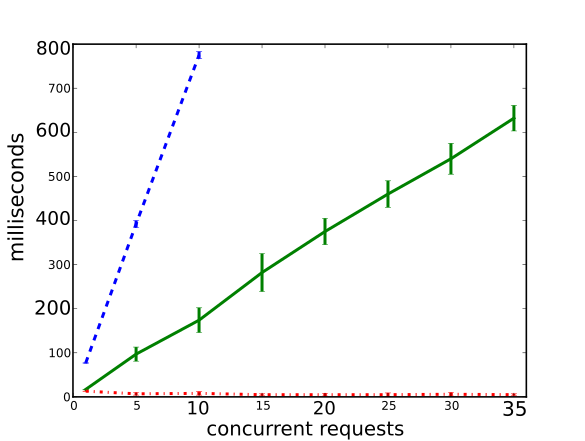
\includegraphics[width=3in]{images/device_comparison.png}
% \label{fig:deviceCompatison}
% \caption{Time measurement comparison among XBee sensors, FoxG20 and a regular computer}
% \end{figure}




\InsertFig{device_comparison}{fig:deviceComparison}{
  Response times measured in different embedded devices
}{
  The dash-dotted line represents the regular computer, the solid line the FoxG20 and the dashed line the XBee.
}{0.7}{}


\begin{table}[htbp]
    \caption{Mean of the measurements taken in different devices with the standard deviation ($\sigma$) in parenthesis.}
    \centering
    \begin{tabular}{|c|c|c|c|}
      \hline
      Concurrent & XBee & FoxG20 & Regular \\
      requests   &  & &  computer \\
      \hline
      1  &  77 (1)	&  17 (0)  &  13 (0) \\
      5  & 392 (8)	&  97 (16) &   7 (3) \\
      10 & 775 (8)	& 174 (28) &   8 (4) \\
      15 &  -	& 282 (43) &   5 (2) \\
      20 &  -	& 375 (30) &   5 (3) \\
      25 &  -	& 460 (30) &   5 (4) \\
      30 &  -	& 540 (35) &   6 (4) \\
      35 &  -	& 632 (29) &   5 (2) \\
      \hline
    \end{tabular}
    \label{tab:timeMeasures}
\end{table}
%\section{Conclusion}
% 2. Comparativa
\label{sec:tsc_wot_conclusion}

% 5. otra forma de aunar las ventajas de ambos? => construir un TSC compatible con WoT (on top of that) <= integración profunda
%	Ventajas:
%		+ interoperable with other semantic WoT systems
%		+ syntactic services can still be provided using a different type of representation => WoT
%		+ promote indirect communication style => abstraction for the developer (does not care about manually discovering interfaces)
%	Problemas:
%		+ necesitas out-of-the-band conocimiento? API fija?
% esto trae problemas: cap 4 y cap 5


This chapter compares two different resource oriented approaches for the \acl{iot}: \acl{wot} and \acl{tsc}.
\ac{wot} seems to scale in a better way thanks to the underlying HTTP protocol, while \ac{tsc} performs the discovery process among locally available network-connected objects in a seamless way.
The first one is more human oriented and the second one relies on the Semantic Web capabilities to exchange a machine processable data.
Furthermore, the second one is ideal to easily configure intranets of network connected objects whilst the first one can easily bridge those intranets configuring global multi-site IoT ecosystems.

We deem that both approaches can win much from their combination since the weaknesses of one are outweighed by the strengths of the other.
Hence, they can be combined to offer a more scalable, machine and human processable solution that offers better cooperation possibilities among internet-connected objects and thus aid users in their daily activities.
As a simple proof of this hypothesis, a scenario employing \ac{wot} to export each space data to the outer world and \ac{tsc} to enable seamless and automatic configuration of heterogeneous devices on local networks has been presented.